%%%%%%%%%%%%%%%%%%%%%%%%%%%%%%%%%%%%%%%%%%%%%%%%%%%%%%%%%%%%%%%%%%%%%%
% How to use writeLaTeX: 
%
% You edit the source code here on the left, and the preview on the
% right shows you the result within a few seconds.
%
% Bookmark this page and share the URL with your co-authors. They can
% edit at the same time!
%
% You can upload figures, bibliographies, custom classes and
% styles using the files menu.
%
%%%%%%%%%%%%%%%%%%%%%%%%%%%%%%%%%%%%%%%%%%%%%%%%%%%%%%%%%%%%%%%%%%%%%%

\documentclass[12pt]{article}

\usepackage{sbc-template}

\usepackage{graphicx,url}

\usepackage{algorithm,algorithmic}
\usepackage{listings}

\makeatletter
\renewcommand{\ALG@name}{Algoritmo}
\renewcommand{\refname}{Refer\^encias}
\makeatother


\usepackage{algpseudocode}


%\usepackage[brazil]{babel}   
\usepackage[utf8]{inputenc}  
     
\sloppy

\title{Uma análise comparativa entre algorítimos estáticos para balanceamento de carga em redes SDN em ambiente IoT}

\author{Anselmo L. E. Battisti\inst{1}, Gabriel Carrara\inst{1}}

\address{Instituto de Computação -- Universidade Federal Fluminense (UFF)}

\begin{document} 

\maketitle

\begin{resumo} 
As redes de comunicação de dados são fundamentais para a implantação das Cidades Inteligentes. Além delas fornecerem conectividade aos cidadãos, é a partir da infraestrutura de redes que os inúmeros sensores enviam dados para as centrais de processamento. Um dos requisitos fundamentais para a implantação de uma infraestrutura de IoT é a escalabilidade da rede de transmissão de dados. Uma das alternativas para melhorar a escalabilidade de uma rede é a implantação de mecanismos de balanceamento de carga. Nesse trabalho foram analisadas três técnicas diferentes para balanceamento estático do tráfego em uma rede SDN. Foi observado que o balanceamento utilizando \textit{Weighted Round Robin} (WRR) foi superior em  cenários com larguras de banda desbalanceadas, ao passo que em redes com larguras de bandas balanceadas o algorítimo Round Robin (RR) foi mais eficiente.
\end{resumo}

\begin{abstract}
    
\end{abstract}

\section{Introdução}

Diversas tecnologias vem sendo estudadas a fim de melhorar a qualidade de vida da população. Dentre elas podemos citar as cidades inteligentes; internet da coisas (IoT); redes definidas por software (SDN). Nesse trabalho será realizada a comparação entre três algorítimo de balanceamento de cargas. Esses algorítimos serão implementados dentro do controlador SDN, dorante chamado de \textit{Load Balancer}. Esse tipo de estratégia pode melhorar largura de banda bem como o tempo de acesso de dispositivos IoT a recursos em uma rede SDN. 

Existem dois tipos de algorítimos de balanceamento de carga, sendo eles estáticos e dinâmicos. Nesse trabalho serão comparados três algorítimos estáticos, sendo eles: Random; Round Robin (RR) e \textit{Weighted Round Robin} (WRR). A comparação será realizada em três cenários diferentes de disponibilidade de largura de banda entre os servidores e o \textit{Load Balancer}.

Desta forma, formula-se a seguinte hipótese a ser investigada nesse trabalho:

\textit{h0: Não existe diferença significativa entre os tempo de resposta e a taxa de download entre os algorítimos de balanceamento de carga estáticos Random; RR e WRR.}

O presente trabalho está estruturado da seguinte forma. Na sessão do referencial teórico será apresentada uma visão geral sobre as principais tecnologias envolvidas na concepção deste trabalho. Em seguida será apresentada o método adotado nessa pesquisa, em seguida serão apresentados os resultados obtidos. Ao final, serão apresentadas as considerações final do trabalho e possíveis extensões que o mesmo pode receber.

\section{Referencial Teórico}

Nessa sessão será apresentada uma visão geral sobre os principais conceitos e tecnologias abordados nesse trabalho. Os principais temas são: Cidades Inteligentes; Internet da Coisas. SDN e balanceamento de carga. Também apresentaremos nessa sessão alguns trabalhos que já realizaram comparações entre esses algorítimos. 

\subsection{Cidades Inteligentes}

O crescente aumento da população urbana demandou ao longo da história que novas tecnologias fossem desenvolvidas para pudesse existir bem estar social. Em seu artigo \cite{Caragliu2011} apresenta uma agenda com alguns tópicos estratégicos que devem ser analisados para que uma cidades possa ser chamada de inteligente. No Brasil a realidade do aumento da população urbana também é constatada de acordo com o \cite{IBGE2011}. Sendo assim novas tecnologias devem ser estudadsa e implementadas também no Brasil.

Além dos aspectos sociais apontados por \cite{Caragliu2011}, também podemos analisar as cidades inteligentes sobre aspectos mais técnicos da sua implementação. \cite{Gharaibeh2017} apresenta em seu trabalho uma visão geral sobre as principais tecnologias que permitiriam a criação deste tipo de ambiente. Dentre elas, podemos destacar: Internet das coisas; gestão e segurança dos dados; virtualização de funções de rede; computação nas nuvens e redes definidas por software. 

O simples uso da da tecnologia não garante que uma cidade seja inteligente. Em seu trabalho \cite{Anttiroiko2014} propõe uma classificação para cidades inteligentes onde existe uma correlação direta entre o emprego adequado das tecnologias da informação com a qualidade de vida dos sujeitos. Como tônica de sua pesquisa ele apresenta que a comunicação entre os sistemas é primeiro degrau que se deve alcançar para que uma cidade possa ser inteligente.

Nesse trabalho estamos buscando mecanismos que permitam que as redes de comunicação de uma cidade inteligente sejam escaláveis. Essa escalabilidade pode ser alcançada de diversas formas, aqui, estamos interessados no balanceamento de carga. Além da escalabilidade o balanceamento de carga pode aumentar também a disponibilidade dos recursos existentes.

\subsection{Internet das Coisas}

Com o aumento da disponibilidade de mecanismos de transmissão de dados, tais como: WIFI, bluetooth, RFID, Li-Fi, 5G. É possível iniciar a coleta de dados de locais e ambientes onde antes não era possível. \cite{Ashton2009}  em 1999 em uma palestra na P&G foi um dos primeiros a utilizar o termo Internet das Coisas (IoT). Ele  acredita que a internet das coisas representa uma maneira de automatizar a coleta de informações do mundo real, uma vez que o ser humano tem limitação de tempo atenção e precisão quanto a coleta desse tipo de dados. IoT pode mudar o mundo mais drasticamente do que a mudança ocorrida pelo desenvolvimento e posterior popularização da Internet tradicional. 

Em seu trabalho \cite{Aziz2016} propõe uma metodologia específica para a elicitação de requisitos para o que ele chama de \textit{Smart Space}. Para eles, um \textit{Smart Space} é um ambiente que fornece algum tipo de inteligência utilizando para tanto estrutura de IoT. Em um mesmo espaço físico podem existir diversos \textit{Smart Space} uma vez que cada \textit{Smart Space} pode ser desenvolvido para oferecer um conjunto de recursos e funcionalidades para os habitantes do local. Nesse contexto é importante perceber a cidade inteligente como um conjunto de \textit{Smart Space} cujos requisitos de rede podem variar e, portanto, podem beneficiar-se dos algorítimos de balanceamento de carga.

O uso de \textit{Web Services} como elemento de troca de dados entre dispositivos IoT e servidores centralizados de coleta de dados foi estudado por \cite{Glombitza2010}. Mesmo em seu estágio embrionário já se considerava o uso de arquitetura cliente servidor para elaboração em ambientes IoT. Nesse trabalho tanto o balanceamento de carga será realizado entre servidores HTTP a fim de simular esse cenário.

\subsection{Redes Definidas por Software (SDN)}

As redes de computadores passaram por diversas formas de organização ao longo das últimas décadas. Recentemente, uma estratégia que vem sendo debatida pela comunidades acadêmica e implantada pela indústria são as SDN. Elas são uma nova abordagem para o gerenciamento de redes de computadores. Nelas, o hardware de encaminhamento de pacotes (\textit{switch}) conta com o apoio de um elemento centralizador chamado \textit{controller} que analisa os pacotes e decide sobre de que maneira os pacotes devem ser encaminhados. 

SDN é um tipo de rede abstrata que permite uma otimização dos recursos da infraestrutura de redes tanto no que diz respeito à eficiência do uso dos diversos dispositivos e meios de transmissão de rede disponíveis, como dos recursos humanos. Segundo os autores, essas duas situações são otimizadas usando SDN pois é possível balancear a carga da rede, utilizando assim melhor os recursos disponíveis, além disso, esse balanceamento pode ser feito via software o que permite a um operador gerenciar um número maior de redes independentemente do local onde elas se encontram. SDN torna o processo de gerenciamento da infra de rede um processo muito mais relacionado com a configuração de software do que de configuração de hardware físicos, como originalmente era feito. Essa abordagem segundo  \cite{Sezer_et_al_2013} apresenta alguns pontos importantes que devem ser analisados. Alguns deles são:

 \begin{itemize}
   \item Performance x flexibilidade:  CPU são mais flexíveis porém mais lentos do que circuítos de propósito específico usados nos encaminhadores de pacotes;
   \item Escalabilidade: existe um controlador central acessado por todos os encaminhadores de pacotes, isso pode limitar a escalabilidade da rede; 
   \item Segurança: como garantir em um ambiente com múltiplos usuários que a criação de novos fluxos não alterem os fluxos de outros usuários? Como tratar ataques de DDoS em um ambiente de propósito geral onde o controlador precisa analisar todos os pacotes que chegam até ele?
   \item Interoperabilidade: será necessária a introdução de novos protocolos que permitam a operação em paralelo de redes tradicionais e SDN em ambiente híbridos.
 \end{itemize}


Um ponto crítico do uso de SDN é a existência de um ponto de falha central. Caso o \textit{controller} não esteja operacional, toda a rede ficará indisponível. Com o objetivo de aumentar a disponibilidade de uma rede SDN, \cite{Dixit2013} propõe uma estrutura onde existam múltiplos \textit{controllers} em uma rede SDN.

O uso de SDN em ambientes IoT vem sendo estudada. Em seu artigo \cite{7366932} apresenta uma abordagem chamada \textit{Black SDN}. O objetivo dessa tecnologia é aumentar a segurança em redes cujos dispositivos na maior parte do tempo esteja, hibernando e, apenas utilizem a rede em algum momento em particular. Os autores advogam que a tecnologia SDN permite a resolução de dois grandes problemas, o primeiro diz respeito a privacidade dos dados e o segundo diz respeito a localização dos recursos da rede. Os autores argumentam que uma das formas de mitigar a incidência de ataques sobre a privacidade dos dados é utilizar protocolos de segurança que criptografem os dados e metadados, além disso é necessário também criptografar os dados da camada de redes. Já para o problema de localização dos dispositivos eles sugerem que exista um controlador central que coordene o processo de troca de trafego entre os dispositivos. Com essa abordagem existe um mascaramento da origem e do destino do pacote, tornando assim anônima o processo de troca de dados entre dispositivos.

O artigo \cite{6819050} propôs uma nova arquitetura distribuída baseada no OpenFlow. Essa arquitetura tenta garantir a QoS fim-a-fim que é muito desejada em aplicações multimídia. A base da arquitetura proposta está na coleta e organização da topologia da rede e também do seu estado, tanto intra como inter domínios (AS), de tal forma que seja possível classificar o fluxo de dados de acordo com o nível de QoS necessário para que o usuário final fique satisfeito. Em uma cidade inteligente garantir qualidade de serviço é uma das tarefas centrais do administradores da rede.

O artigo \cite{Li2016} apresenta uma proposta de arquitetura horizontal para IoT utilizando SDN como meio de controle dos fluxos de dados. Segundos os autores, existe falta de interoperabilidade entre os diversos fabricantes de hardware e software para IoT, isso gera uma verticalização da infra-estrutura, ou seja, um tipo de sensor funciona para um certo tipo de domínio ou aplicação mas não para outro. Esse cenário, entre outras coisas gera dificuldade em inovação.  A proposta apresentada fornece mecanismos que permitem a interoperabilidade de dados, dispositivos e softwares pelo uso dos controladores SDN.

O uso de uma estrutura de redes desenvolvida com SDN permite, entre outras coisas, escalabilidade e a capacidade de inovação necessária dentro do contexto de redes que é necessário em uma cidade inteligente. Na próxima sessão falaremos sobre de que maneira o balanceamento de carga pode ser implementado em uma SDN e de que maneira isso afeta a escalabilidade de uma rede.

\subsection{Balanceamento de Carga}

O balanceamento de carga em redes de computadores vem sendo estudado há algumas décadas. Em seu trabalho seminal \cite{Stentz1988} apresenta a formulação do problema e também um algorítimo para calcular o quão balanceada uma rede está.

Balanceamento de carga em redes de computadores segundo \cite{Peter2012} consiste em dividir o tráfego da rede entre diversos servidores sem que o usuário final perceba que essa divisão está acontecendo, como pode ser visto na  Essa visião equitativa o tráfego de uma rede deve seguir critérios estabelecido pelos gestores da rede. Algumas métricas que podem ser utilizadas para a definição do problema de balanceamento da rede são: tempo de resposta; vazão; perda de pacotes; custo; segurança da informação; etc.

A abordagem apresentada por \cite{Peter2012} utiliza um \textit{load balancer} no modo tradicional, como pode ser visto na Figura \ref{fig:balanceamento_carga_tradicional}. Nessa abordagem, existe um servidor a frente do switch interno da rede que faz o papel de ponte entre cada um dos servidores de conteúdo e o cliente que solicita o dado. Essa abordagem tradicional requer um servidor específico para o balanceamento do tráfego, em uma SDN, podemos usar o controlador para essa finalidade.

Nesse artigo estamos interessados em avaliar e analisar o balanceamento da carga da rede a partir da perspectiva do controlador de uma rede SDN. O controladores naturalmente já recebe solicitação de roteamento dos diversos \textit{switches} da rede, sendo assim podemos usar as demandas do tipo \textit{packet-in} para disparar algoritmos para o adequado balanceamento da rede.

\begin{figure}[ht]
\centering
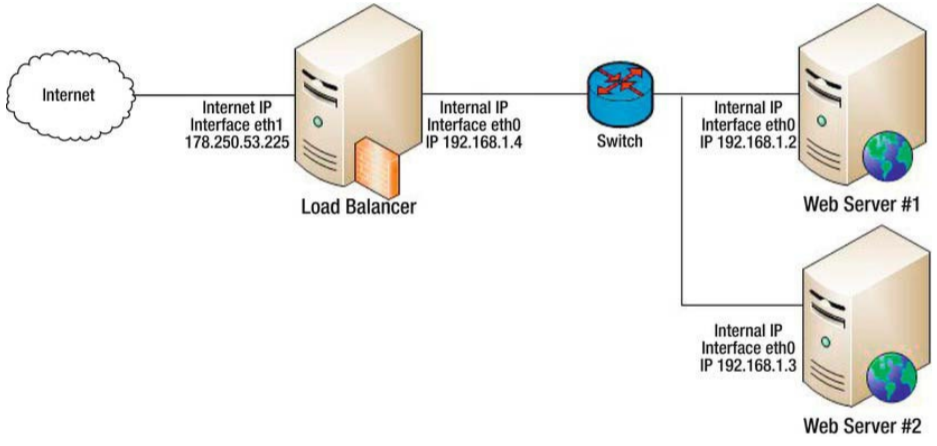
\includegraphics[width=0.8\textwidth]{images/load_balance.png}
\caption{Balanceamento de carga no modelo tradicional \cite{Peter2012}}
\label{fig:balanceamento_carga_tradicional}
\end{figure}

Podemos dividir os algorítimos de balanceamento de carga em dois grupos, os estáticos e os dinâmicos. Os algorítimos estático levam em consideração apenas os dados definidos no momento da sua concepção, parametrização e inicialização, ou seja, depois do início da sua operação o seu comportamento é baseado naquilo que ele sabia anteriormente, o Round Robin é um exemplo deste tipo de algorítimo. Já os algorítimos dinâmicos tomam a decisão sobre para quem enviar um processo de acordo com o estado atual da rede, nesse caso o \textit{load balancer} precisa obter informações sobre os servidores e links a fim de definir o destino de uma solicitação.

Nesse trabalho serão avaliados três diferentes algorítimos de balanceamento de carga. Esses algorítimos serão avaliados em três cenários distintos que podem ocorrer em uma cidade inteligente. Na próxima sessão será apresentado o método de pesquisa utilizado nesse trabalho.

\section{Apresentação do Método}

Nessa sessão serão apresentados os procedimentos metodológicos utilizados na elaboração e condução dos experimentos. Segundo \cite{Sampieri2013} um experimento consiste em um ato investigativo onde o pesquisador manipula variáveis independentes entre grupos distintos e homogêneos de tal forma que os efeitos dessa manipulação possam ser observados e correlações sejam estabelecidas.

Nesse experimento, a fim de testarmos a hipótese h0, a variável independente manipulada foi a largura de banda entre o SDN \textit{load balancer}. Para tanto, foi utilizado o teste de hipótese Kruskal-Wallis, um teste não paramétrico onde k populações são testadas a fim de analisar se as médias da variável independente são iguais, exatamente como nossa hipótese h0. 

A fim de maximizar a validade dos dados obtidos no experimento, alguns cuidados foram tomados durante a execução do experimento foram:

\begin{enumerate}
    \item Antes da execução de cada um dos experimentos tanto o mininet como o controlador POX foram reiniciados a fim de garantir que dados em cache do experimento anterior não afetassem o resultado do experimento atual;
    \item Foram desativadas atualizações automáticas de pacotes;
    \item A implementação tanto do algorítimo de RR como o WRR tinham a complexidade $\mathcal{O}(n)$. Essa complexidade é a mesma do algorítimo Random já implementado no \textit{script} utilizado como base inicial deste trabalho.
\end{enumerate}

Existem diversas ferramentas para a realização de testes em servidores HTTP, tais como: httperf; openload; autobench; \textit{ab}, entre outras. Para este experimento a coleta dos dados foi realizada utilizando a ferramenta de testes de servidores HTTP desenvolvida pela \textit{Apache Software Fundation} chamada \textit{ab}. Ela foi escolhida pois a sua mantenedora possui reconhecimento pela indústria e também pela academia no desenvolvimento e testes de servidores HTTP. Os parâmetros utilizados na execução do \textit{ab} foram os seguintes:

\begin{itemize}
    \item \textbf{-n}: indica o número de vezes que o teste será executado. Nesse experimento o valor foi definido como 30 para todos os cenários testados;
    \item \textbf{-c}: indica o número de clientes concorrentes que serão executados, esse valor foi definido como 5, um para cada cliente em nosso experimento;
    \item \textbf{-r}: indica que caso haja uma desconexão por parte do servidor HTTP o teste não deve parar de ser executado;
    \item \textbf{url}: em cada um dos três experimentos foram testadas urls com tamanhos de retornos diferentes, os valores variaram entre 500Kb e 5000Kb com intervalo de 500Kb entre cada arquivo.
\end{itemize}

Sendo assim, em cada um dos experimentos, para cada algorítimo testado foram executadas 30 chamadas para cada um dos 10 tamanhos diferentes de arquivo totalizando 2700 coletas de dados. Após a execução dos testes, os arquivos gerados pelo \textit{ab} foram processados a fim de extrair apenas os dados necessários para o teste da hipótese h0.

Os dados foram processados e interpretados utilizando a linguagem de programação Python na versão 3.7. Os testes de hipótese foram realizados utilizando a linguaram R sendo essa processada a partir do software R Studio versão 1.1.453. 

\section{Técnicas de Balanceamento de carga analisadas}

Nesse trabalho foram testadas três técnicas distintas de balanceamento estático de carga em uma rede SDN, sendo eles:

\begin{itemize}
    \item Aleatório: nesse algorítimo o controlador SDN escolhe de forma aleatoria qual será o servidor responsável pelo processamento de uma solicitação;
    \item Round-Robin: nesse algorítimo o controlador SDN escolhe de forma sequencial qual será o próximo servidor que irá atender uma solicitação. A implementação utilizou uma lista circula para alcançar esse comportamento;
    \item Weighted Round-Robin: nesse algorítimo o controlador SDN escolhe de forma sequencial qual será o próximo servidor que irá atender uma solicitação. A implementação utilizou uma lista circula para alcançar esse comportamento, porém, nesse cenário cada servidor tem pesos diferentes, ou seja, servidores com peso maior receberão mais requisições ao passo que servidores com peso menor receberão menos requisições,
\end{itemize}

\subsection{Estrutura da rede utilizada}

A fim de testar as três estratégias para o balanceamento da carga, Random, RR e WRR, foi montada uma estrutura que simula um ambiente típico de uma cidade inteliente com servidores distribuídos e com larguras de bandas variadas disponíveis. Nesse cenário existem vários servidores rodando um cliente HTTP, cada cliente tem o mesmo conteúdo, e cada servidor é responsáveis por responder diversos clientes. Para os clientes, essa arquitetura de multi-servidores é transparente, ou seja, todos os clientes fazem a requisição para um único ponto, seja um IP ou URL, nesse local existe um \textit{load balancer} que fica responsável por enviar o fluxo de dados para um dos servidores, essa escolha é feita no algorítimo de balanceamento de carga dentro do \textit{load balancer}. 

Na Figura \ref{fig:rede_proposta} pode ser vista a estrutura elaborada para a execução dos experimentos. Cada um dos clientes realiza requisições para o \textit{load balancer} e ele tem a função de invocar o servidor adequado para o processamento da solicitação. Tanto os clientes como os servidores foram simulados utilizando o mininet.

\begin{figure}[ht]
\centering
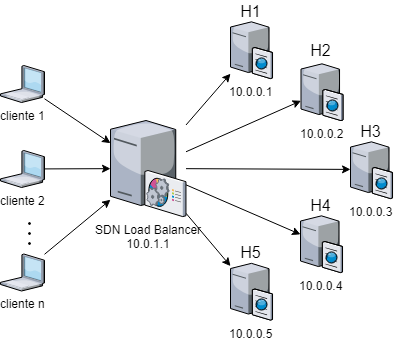
\includegraphics[width=0.6\textwidth]{images/network.png}
\caption{Estrutura da rede utilizada para a realização dos testes}
\label{fig:rede_proposta}
\end{figure}

A largura de banda dos links entre todos os clientes e o \textit{load balancer} foi mantida exatamente a mesma, 100 Mbits, durante os experimento. Já entre o \textit{load balancer} e os servidores foram estabelecidos valores diferentes de largura de banda de acordo com cada experimento como pode ser visto na Tabela \ref{largura_banda}. O objetivo de estabelecer valores diferentes de links para cada um dos servidores teve por objetivo simular o comportamento de cada algorítimo em cenários distintos de conectividade entre o \textit{load balancer} e os servidores.

\begin{table}[]
\centering
\caption{Largura de banda de cada servidor em cada um dos experimentos, valores em MBits/seg}
\label{largura_banda}
\begin{tabular}{llllll}
 & H1 & H2 & H3  & H4 & H5 \\\hline
Experimento 1                  & 1  & 2  & 4   & 8  & 16 \\
Experimento 2                  & 10 & 10 & 10  & 10 & 10 \\
Experimento 3                  & 5  & 5  & 7.5 & 10 & 10
\end{tabular}
\end{table}

Como pode ser visto na Tabela \ref{largura_banda} foram testadas três diferentes configurações de largura de banda entre o servidor e o \textit{load balancer}. No experimento 1, foram definidas larguras de banda com variação exponencial, esses valores foram escolhidos a fim de simular ambientes onde os servidores que rodam na borda da rede de uma cidade inteligente tenham menos largura de banda disponível que os servidores que rodam mais ao centro da rede. O experimento 2 foi planejado para testar um ambiente onde todos os servidores possuíssem a mesma largura de banda. Já no experimento 3, metade dos servidores possuíam metade da banda dos outros servidores, simulando assim um cenário onde um upgrade da rede poderia estar ainda em curso. O objetivo de cada experimento é avaliar o potencial de cada algorítimo em cenários distintos de largura de banda.

\subsection{Hardware de Teste}

A fim de tornar os resultados dos testes fidedignos, optou-se por implantar o ambiente de teste em uma máquina virtual dedicada exclusivamente para a execução dos testes. A máquina foi hospedada em um datacenter da Digital Ocean. As configurações da mesma são as seguintes: 1GB de memória RAM; Processador Intel(R) Xeon(R) CPU E5-2650 v4 @ 2.20GHz.

O servidor roda o sistema operacional Ubuntu 18.04.1 LTS. Foram desativados recursos como atualização de pacotes para evitar que processos estranhos pudessem interferir nos resultados. Além disso, foram analisados os logs durante a coleta dos dados do experimento a fim de garantir que processos externos ao experimento não estavam consumindo recursos de hardware.

\subsection{Software utilizados}

A rede foi simulada utilizando o a plataforma mininet na versão 2.3.0d4. O controlador escolhido para a execução dos testes foi o POX em sua versão 0.5.0 (eal). A escolha do tanto do mininet como do controlar POX deram-se em virtude da sua facilidade de aprendizado permitindo assim uma rápida prototipação do amviente dos testes.

A implementação dos algorítimos de balanceamento de carga foi feito utilizando como referência o \textit{script} pré-instalado do POX chamado "ip\_loadbalancer\.py" desenvolvido por James McCauley. Em sua versão original o \textit{script} implementa o balanceamento de carga utilizando o sorteio aleatório do servidor que será responsável pelo tratamento da requisição do cliente. Para a execução dos experimentos esse \textit{script} foi modificado para dar suporte ao algorítimo RR e também ao WRR a fim de realizar as comparações desejadas. As modificações realizadas estão disponíveis no github no link https://github.com/anselmobattisti/loadbalance\_tests.

Na próxima sessão serão apresentados os resultados obtidos com os experimentos realizados. Além disso, serão apontadas alguma evidências empíricas que apontam para a variação do resultado tanto em função do algorítimo escolhido como do cenário estudado. 

\section{Resultados Obtidos}

Nessa sessão serão apresentados os resultados obtidos em cada um dos experimentos realizados. Serão analisados o tempo médio de resposta e também taxa de download obtida em cada um dos cenários e em cada um dos algorítimos.

\subsection{Experimento 1}

Como apresentado na Tabela \ref{largura_banda}, o experimento 1 consiste na simulação de uma rede onde a larguras de banda definidas entre os servidores e o \textit{load balancer} tem uma variação exponencial. Esses valores foram escolhidos a fim de simular ambientes onde os servidores que rodam na borda da rede de uma cidade inteligente tenham menos largura de banda disponível do que os servidores que rodam mais ao centro da rede. Os valores escolhidos para as larguras de banda são relativamente baixos com o objetivo de testar os piores casos de conectividade. 
A figura \ref{fig:exp1_t} mostra a relação existente entre o tamanho do arquivo e o tempo de resposta obtido. Nesse cenário podemos observar que o algorítimo com o melhor desempenho foi o Weighted Round Robin. Nesse experimento foi dada maior prioridade para o servidor h5, como nesse experimento esse servidor possuía a maior largura de banda o tempo de resposta foi o menor. 

\begin{figure}[ht]
\centering
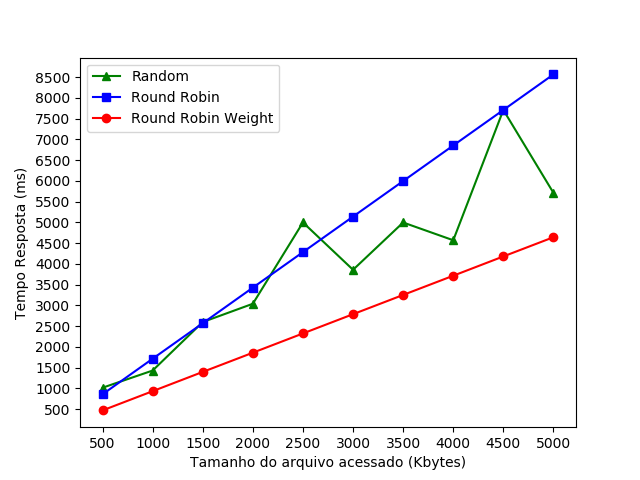
\includegraphics[width=0.6\textwidth]{images/exp1_time.png}
\caption{Relação entre o tamanho do arquivo e o tempo de acesso.}
\label{fig:exp1_t}
\end{figure}

Já em relação a taxa de download, Figura \ref{fig:exp1_b}, podemos observar que direcionando a maior parte do fluxo para o servidor h5 afetou positivamente essa métrica. Esse tipo de experimento mostra que de forma geral, encaminhar fluxos para servidores com maior largura de banda pode melhorar a experiência do usuário final em relação ao uso de um determinado serviço em uma cidade inteligente.

\begin{figure}[ht]
\centering
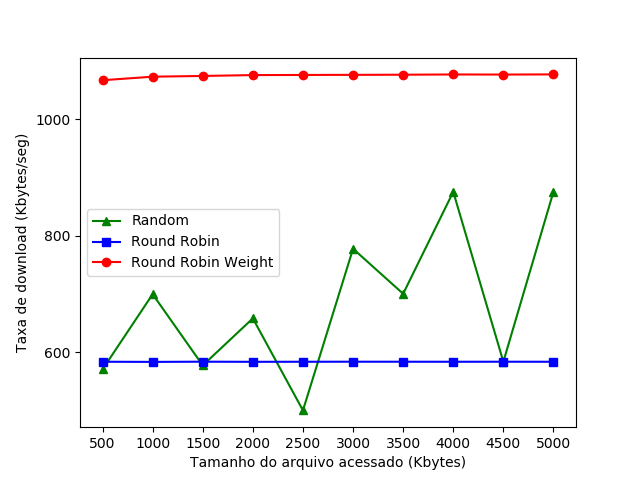
\includegraphics[width=0.6\textwidth]{images/exp1_banda.png}
\caption{Relação entre o tamanho do arquivo e a taxa de download.}
\label{fig:exp1_b}
\end{figure}

\subsection{Experimento 2}

No experimento 2 o link entre todos os servidores e o Load Balancer foram mantidos exatamente iguais, 10 MBits/s, simulando assim um cenário de homogeneidade de largura de banda disponível. De forma intencional, o servidor H4 no algorítimo Round Robin Wighted recebeu um fluxo 4x maior do que os demais servidores. Essa modificação mostrou que em um ambiente homogêneo a distribuição equitativa proposta pelo algorítimo Round Robin foi a mais interessante e, a priorização de fluxos para um determinado servidor apresentou um pior desempenho.

Outro fator digno de nota é que, mesmo em um cenário homogêneo, o algorítimo Random teve um desempenho pior que o algorítimo Round Robin pois, em um sorteio aleatório, pode haver um desbalanceamento da distribuição da carga de trabalho, como pode ser visto na Figura \ref{fig:exp2_t}.

\begin{figure}[ht]
\centering
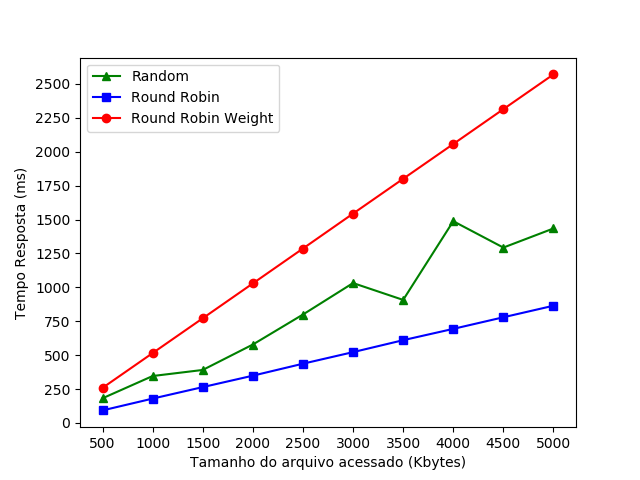
\includegraphics[width=0.6\textwidth]{images/exp2_time.png}
\caption{Relação entre o tamanho do arquivo e o tempo de acesso.}
\label{fig:exp2_t}
\end{figure}

Já em relação a taxa de download, Figura \ref{fig:exp2_b}, podemos observar que direcionando de forma homogênea os dados obteve-se o melhor resultado. Esse cenário mostra que em um ambiente cuja largura de banda seja homogênea é interessante distribuir também de forma homogênea as requisições entre os servidores disponíveis.

\begin{figure}[ht]
\centering
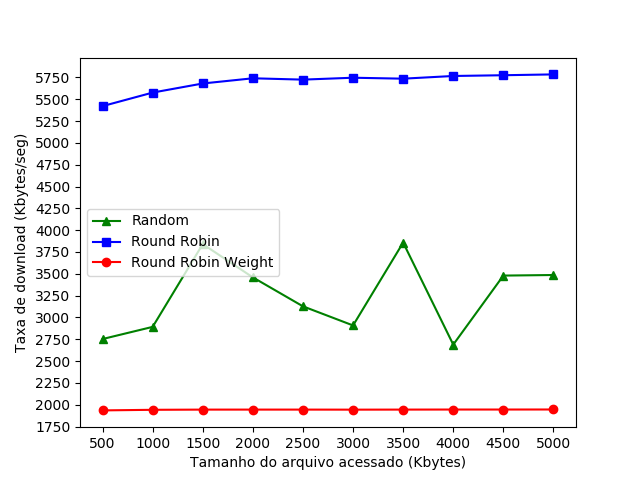
\includegraphics[width=0.6\textwidth]{images/exp2_banda.png}
\caption{Relação entre o tamanho do arquivo e a taxa de download.}
\label{fig:exp2_b}
\end{figure}

\subsection{Experimento 3}

Já no experimento 3, a metade dos servidores possuíam metade da banda dos outros servidores. Essa configuração simula um cenário onde um upgrade da rede poderia estar ocorrendo. Ou seja, parte da rede continuaria com uma largura de banda menor e a outra parte da rede com uma largura de banda maior. 

Nesse cenário, podemos observar na Figura \ref{fig:exp3_t} uma pequena variação entre os algorítimos Round Robin e Weighted Round Robin. Nesse experimento foi atribuída duas vezes mais chances de acesso há um servidor com maior largura de banda do que aos servidores com menor largura de banda. Os resultados apontam que em um cenário onde a largura de banda é maior do que o tamanho dos arquivos que estão sendo trafegados o uso de priorização de tráfego praticamente não afeta a operação.

\begin{figure}[ht]
\centering
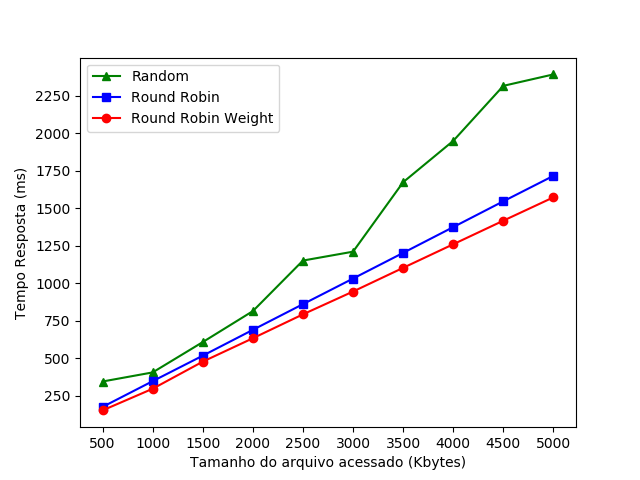
\includegraphics[width=0.6\textwidth]{images/exp3_time.png}
\caption{Relação entre o tamanho do arquivo e o tempo de acesso.}
\label{fig:exp3_t}
\end{figure}

Já em relação a largura de taxa de download, Figura \ref{fig:exp2_b}, podemos observar uma invariabilidade dos valores tanto no algorítimo Round Robin quanto no Weighted Round Robin. 

\begin{figure}[ht]
\centering
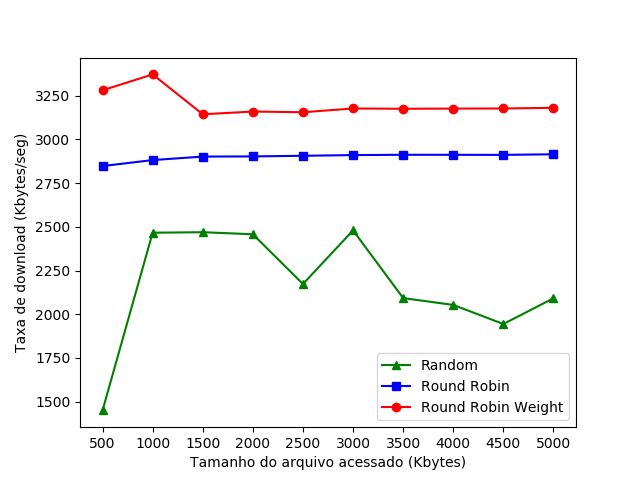
\includegraphics[width=0.6\textwidth]{images/exp3_banda.png}
\caption{Relação entre o tamanho do arquivo e a taxa de download.}
\label{fig:exp3_b}
\end{figure}

\subsection{Análise Comparativa}

A fim de testar a hipótese h0, foi executado o teste de hipótese não paramétrico  Kruskal-Wallis. O objetivo era verificar se as médias da variável independente eram iguais. Os resultados apontaram que com um nível de confiança de 95\% não podemos aceitar a hipótese h0 que diz que as médias são iguais, sendo assim, podemos inferir que o uso de diferentes algorítimos de balanceamento em diferentes cenários pode trazer modificações significativas tanto no que diz respeito a taxa de download como no tempo de acesso.

De forma geral os experimentos mostraram que em ambientes homogêneos o uso do algorítimo de balanceamento Round Robin, que distribui o fluxo de forma equitativa entre todos os servidores mostrou-se o mais adequado. Em ambientes hoje existe um desbalanceamento de banda o uso do Weighted Round Robin teve o melhor resultado, em contrapartida, no experimento 2 onde houve uma distribuição inadequada dos fluxos o Weighted Round Robin teve um desempenho pior que o algorítimo aleatório. Podemos então inferir que em cenários onde a largura de banda sofre grande variação ao longo do tempo o uso do Weighted Round Robin pode não ser a melhor escolha uma vez que ele é um algorítimo de balanceamento estático e pode direcionar muitas requisições para um servidor com pouca largura de banda disponível. A tabela \ref{quadro_comparativo} mostra em qual cenário cada algorítimo teve um melhor comportamento.

\begin{table}[]
\centering
\caption{Quando comparativo entre os diferentes cenários e os tipos de algorítimos utilizados}
\label{quadro_comparativo}
\begin{tabular}{lccc}
 & \multicolumn{1}{l}{\textbf{Random}} & \multicolumn{1}{l}{\textbf{Round Robin}} & \multicolumn{1}{l}{\textbf{Round Robin Weighted}} \\\hline
\textbf{Balanceado} &  & X &  \\
\textbf{Desbalanceado} &  &  & X \\
\textbf{Homogêneo} & X & X & 
\end{tabular}
\end{table}

\section{Considerações Finais}

Nesse trabalho foi apresentada a estratégia do balanceamento de carga em uma rede SDN. O balanceamento de carga é um mecanismo de rede que pode minimiza diversos problemas, tais como: uso excessivo de uma única máquina, latência e disponibilidade de um serviço. Foram testadas três estratégias de balanceamento estático, sendo elas: Random. Round Robin e Weighted Round Robin. Os resultados obtidos mostraram que existem diferenças estatísticas significativas entre eles. Sendo assim, podemos inferir que em diferentes cenários o uso do algorítimo mais apropriado pode trazer benefícios, como apontado na Tabela \ref{quadro_comparativo}.

O trabalho realizado por \cite{Kaur2015} também comparou o algorítimo Round Robin com o algorítimo Random em um ambiente similar ao adotado em nossa pesquisa. Os resultados que obtivemos não são similares aos resultados apresentados pelos autores no referido artigo. Infelizmente no artigo citado não havia descrição detalhada sobre a largura de banda utilizada entre os servidores e o \textit{load balancer}, essa pode ser uma das explicações para a discrepância encontrada em nosso experimento.

Todos os testes foram realizados utilizando o controlador POX, sendo assim, não podemos extrapolar esse comportamento para todos os modelos de SDN, porém, acreditamos que os resultados sejam semelhantes uma vez que a complexidade de todos os algorítimo testados é $\mathcal{O}(n)$.

Para permitir a reprodutibilidade do experimento, tanto os \textit{scripts} quanto os dados obtidos e utilizados nas análises estão disponíveis no github, cuja URL é https://github.com/anselmobattisti/IoT-SDN-Loadbalance.

Algorítimos de balanceamento estáticos não levam em consideração nem o estado atual da rede nem a carga dos servidores. Como implementação futura pretende-se desenvolver mecanismos que coletem dinamicamente dados da rede para evitar situações como as apontadas no experimento 2 onde a configuração de balanceamento sobrecarregou um servidor cujo link havia sido modificado para um valor menor do que o esperado.

\bibliographystyle{sbc}
\bibliography{sbc-template}

\end{document}
